\documentclass{article}
\usepackage[letterpaper,top=2cm,bottom=2cm,left=3cm,right=3cm,marginparwidth=1.75cm]{geometry}
\usepackage{graphicx} % Required for inserting images

\usepackage{amsmath}
\usepackage{amsfonts}
\usepackage{graphicx}
\usepackage{setspace}
\usepackage{float}
\usepackage{amsmath}
\usepackage[parfill]{parskip}
\usepackage[colorlinks=true, allcolors=blue]{hyperref}
\usepackage{tcolorbox}
\usepackage{dirtree}
\usepackage{algpseudocode}
\usepackage{algorithm}


\title{CSE305 Concurrent Programming: N-Body simulation project}
\author{Martin Lau, Oscar Peyron, Ziyue Qiu}
\date{\today}

\begin{document}

\maketitle

\section{Introduction}
This document outlines the N-Body simulation project for CSE305, which includes how we approached the problem, our project structure, code breakdown and strategies, and encountered difficulties.

To get started quickly, try typing \texttt{make nbody} in the project directory, and generate a basic gif file.
For information on how to execute the code, check our README file.

For this project, our aim is to be able to simulate systems of bodies with forces interacting with one another in 2D (such as orbiting planets around the solar system with gravitational forces, or with particles interacting with each other with Coulomb forces). This therefore includes two sections:
\begin{enumerate}
    \item Simulation of the N bodies and their evolving states.
    \item Visualization of recorded telemetries into an animated output.
\end{enumerate}

Below is a general view of our project repository file structure. 

\begin{tcolorbox}[title=Project directory summary]
    \dirtree{%
        .1 /.
        .2 output \dotfill Output gif and csv files.
            .3 telemetry.csv.
            .3 out.gif.
        .2 src \dotfill Core files.
            .3 core.cpp/hpp \dotfill Used throughout the entire proj.
            .3 simplesimulation.cpp/hpp.
            .3 barneshutt.cpp/hpp.
            .3 particlemesh.cpp/hpp.
            .3 particlemeshcuda.cpp/hpp.
        .2 py \dotfill Python testing code.
            .3 verifier.py.
        .2 makefile \dotfill Project builder. 
        .2 main.cpp \dotfill Main execution file.
        .2 mainparticlemesh.cpp \dotfill Aux particle mesh run file.
        .2 test\_telemetry.cpp \dotfill Telemetry test file.
        .2 report (PDF, TeX).
    }

\end{tcolorbox}

The work has been split as follows. The arrangement is not defining, as we like to help each other out in different parts. Our files have still been mostly separated to properly separate who worked on what functionalities.
\begin{enumerate}
    \item Martin handles general project structure, core classes, visualization, and the naive and its optimized algorithm implementation.
    \item Ziyue handles the Barnes Hutt algorithm.
    \item Oscar handles the Particle Mesh algorithm implementation.
\end{enumerate}


\section{Core components}

\subsection{Main elements}

There are 3 primary classes defined used throughout our project: \texttt{Vector, Body, System}. These are defined in \texttt{core.cpp/hpp.}
\begin{enumerate}
    \item \texttt{Vector} holds information on a pair of numbers, and also allows for operations with other vectors/scalars (as opposed to using \texttt{std::pair}).
    \item \texttt{Body} holds information on a given particle or body, including its mass, coordinates, velocity, and acceleration. It also contains an update method which updates its position and velocity based on acceleration. 
    \item \texttt{System} stores a collection of bodies and its recorded telemetry from the simulations we are going to do. It also contains the visualization function, which takes its recorded telemetry and outputs an animated file.
\end{enumerate} 
\textit{Note: This organization is heavily inspired from one assignment from CSE306 Computer Graphics.}

Elaborating more on the telemetry stored within the \texttt{System} class, this is stored as a vector of vector of \texttt{Vector}. What a mouthful! Our simulations creates different steps/frames. Each step/frame contains the positions of all bodies inside the system (this is a vector of \texttt{Vector}). To have the entire telemetry, we have a vector of frames, or the aforementioned data structure for the telemetry.

\subsection{Visualization code}

To visualize the code, we opt to create a gif animation after the telemetry is recorded, using the \texttt{ImageMagick/Magick++} libraries. The bulk of the visualization code is located in \texttt{core.cpp} as a method for the \texttt{System} class. As of present, the visualization function works in two steps. First, it creates the frames for the animation, then writes the frames to a gif file. The frame creation is relatively quick, and most of the visualization time is actually spent in one line (\texttt{writeImages(frames.begin(), frames.end(), name)}). 

We will look into further solutions to try and decrease the time taken to create the visualization gifs, like reducing image quality, or the number of frames. 

For testing purposes, there is also a visualizer in \texttt{visualizer.py} which creates a animation using Python's \texttt{matplotlib} library, working significantly faster, allowing us to test the correctness of our telemetries.

\begin{center}
    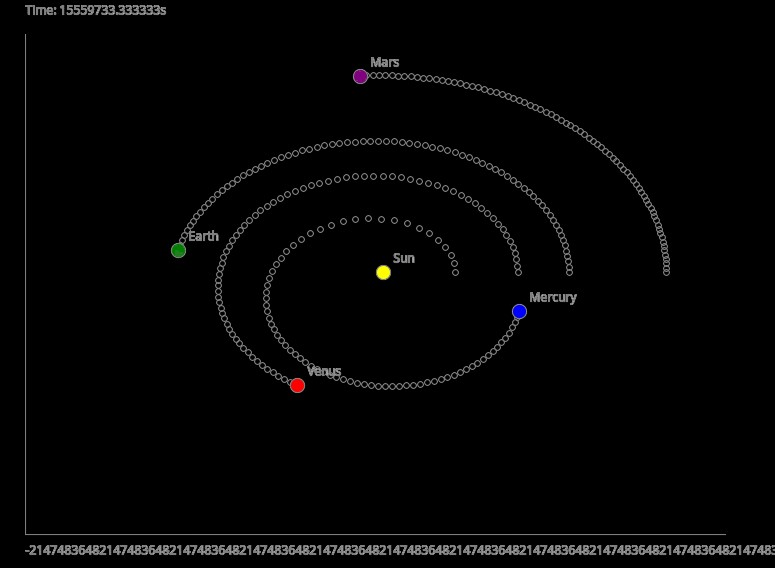
\includegraphics[scale=0.5]{teX/screenshot.jpg}
\end{center}

\section{Naive algorithm}

So far, we have a basic implementation of the naive algorithm without multi threading (most of my time was taken bugfixing core functionalities and getting visualization to work). 

\begin{algorithm}
    \caption{Naive simulation outline}\label{alg:cap}
    \begin{algorithmic}
        \Require System of bodies with masses $m_i$, initial positions $\vec{r}_i$, velocities $\vec{v}_i$
        \Require Time step $\Delta t$, number of steps $N$
        \State telemetry $\gets \emptyset$
        \State telemetry.append(initial positions)
        \For{step $\gets 0$ to $N-1$}
            \For{each body $i$}
                \State $\vec{a}_i \gets \vec{0}$ \Comment{Reset accelerations}
            \EndFor
            \For{$i \gets 0$ to $n-1$}
                \For{$j \gets i+1$ to $n-1$}
                    \State $\vec{F}_{ij} \gets$ ComputeGravitationalForce($body_i$, $body_j$)
                    \State $\vec{a}_i \gets \vec{a}_i + \vec{F}_{ij}/m_i$
                    \State $\vec{a}_j \gets \vec{a}_j - \vec{F}_{ij}/m_j$
                \EndFor
            \EndFor
            \For{each body $i$}
                \State $\vec{v}_i \gets \vec{v}_i + \vec{a}_i\Delta t$ \Comment{Update velocity}
                \State $\vec{r}_i \gets \vec{r}_i + \vec{v}_i\Delta t$ \Comment{Update position}
            \EndFor
            \State telemetry.append(current positions)
        \EndFor
        \Ensure Position history for all bodies stored in telemetry
    \end{algorithmic}
\end{algorithm}

Other aspects (parallelizing the update steps, parallelizing forces computations, avoiding race conditions) will be implemented later on.


\section{Particle Mesh based algorithm}

\section{Barnes Hutt algorithm}


\end{document}